\section{Introduction}
\label{sec:intro}

% \textbf{SARAH - - intro paragraph 1 feels a little all over in the way it addresses creativity — I’d suggest making sure you are specific about whether you are discussing person-focused creativity or artifact-focused creativity.  The last sentence about what you are interested in is key — expand that slightly so we know why it’s difficult to use TTCT.
% \\
% paragraph 2 — “complying” is a weird phrasing here — I’m not sure what that means or why you use that to adapt the TCTT
% \\
% overall I think you need a little more context to start out — instead of jumping into defining creativity history, give half a paragraph on why the work you’re about to do matters.
% }\\

As AI-assisted writing gets more and more popular  \cite{AIassistedWriting1, AIassistedWriting2}, especially in the wake of an enormous movement in the writing industry \cite{WGA}, it is rather timely and urgent to evaluate whether LLMs have the abilities to generate creative content and whether they can assess and critique the creativity of an existing piece.Creativity is often difficult to evaluate because it is a complex, multifaceted concept that is deeply subjective, contextual, and hard to judge objectively. Several empirical studies have been conducted in psychology and cognitive science on the processes through which creativity occurs \cite{kurtzberg2005feeling,cropley2000defining,silvia2008assessing}. Interpretation of the results has led to several possible explanations of the sources and methods of creativity. Eminent psychologist J. P. Guilford drew a distinction between convergent and divergent thinking \cite{guilford1967nature}. Convergent thinking involves aiming for a single, correct solution to a problem, whereas divergent thinking involves the creative generation of multiple answers to a set problem. Divergent thinking is sometimes used as a synonym for creativity in psychology literature or is considered the necessary precursor to creativity \cite{RUNCO2011400}. 

Built on J.P. Guilford's work Ellis Paul Torrance devised one of the widely accepted tests of creativity, \textit{Torrance Tests of Creative Thinking (TTCT)} \cite{torrance1966torrance}, which originally involved simple tests of divergent thinking and other problem-solving skills. Prior work has argued that creative writing constitutes a promising topic for an interdisciplinary conversation about creativity \cite{Doyle1998TheWT}. One of the popular frameworks for Creativity evaluation, TTCT -- typically involves two parts: Verbal and Figural -- measures creativity as a process by testing participants' abilities in dealing with unusual uses of objects, specific situations, or impossibilities. We are however interested in measuring creativity as a product within the realm of short story writing making it difficult to directly rely on TTCT \cite {baer2009assessing}.

In the field of Computer Science, recent work has shown the promise of LLMs in creative writing tasks \cite{mirowski2023cowriting,yang2022re3,lee2022coauthor}, without reaching a consensus on how to evaluate creative writing. Towards this, we design a framework particularly aimed at evaluating creativity as a product by adapting prior work on the evaluation of creativity as a process (Section \ref{design} Design Principle 1 and 2). One of the popular methods for Creativity Evaluation called the \textit{Consensual Assessment Technique} \cite{amabile1982social} states that the most valid assessment of the creativity of an idea or creation in any field is the collective judgment of experts in that field. Similarly in this work, we first collaborate with 8 creative writing experts to collect creativity measures for the evaluation of short fictional stories. 

The evaluation protocol we propose, the Torrance Tests for Creative Writing (TTCW), consists of 14 binary tests organized into the original Torrance dimensions of \textit{Fluency, Flexibility, Originality} and \textit{Elaboration}. In Section~\ref{sec:approach}, we go over the process we followed to create the TTCW by collecting insights from expert creative writers and consolidating them into individual tests. To empirically validate the TTCW as an evaluation method, we create in Section~\ref{sec:data} a benchmark consisting of 48 short stories (12 stories written by professionals, and 36 by various modern LLMs, with 1400 words in average per story). We recruit a new set of 10 experts, again in compliance with CAT, to administer the TTCW on each story, collecting 3 evaluations per story. Based on a total of 2,000+ expert-administered tests, our findings reveal that experts reach moderate agreement on average (Fleiss Kappa $[0.4-0.6]$) across the 14 TTCW tests, and reach strong agreement when considering the aggregated tests (Pearson correlation $0.69$). This confirms the validity of our TTCW for the evaluation of creativity in fictional short stories.

\begin{figure*}
\centering
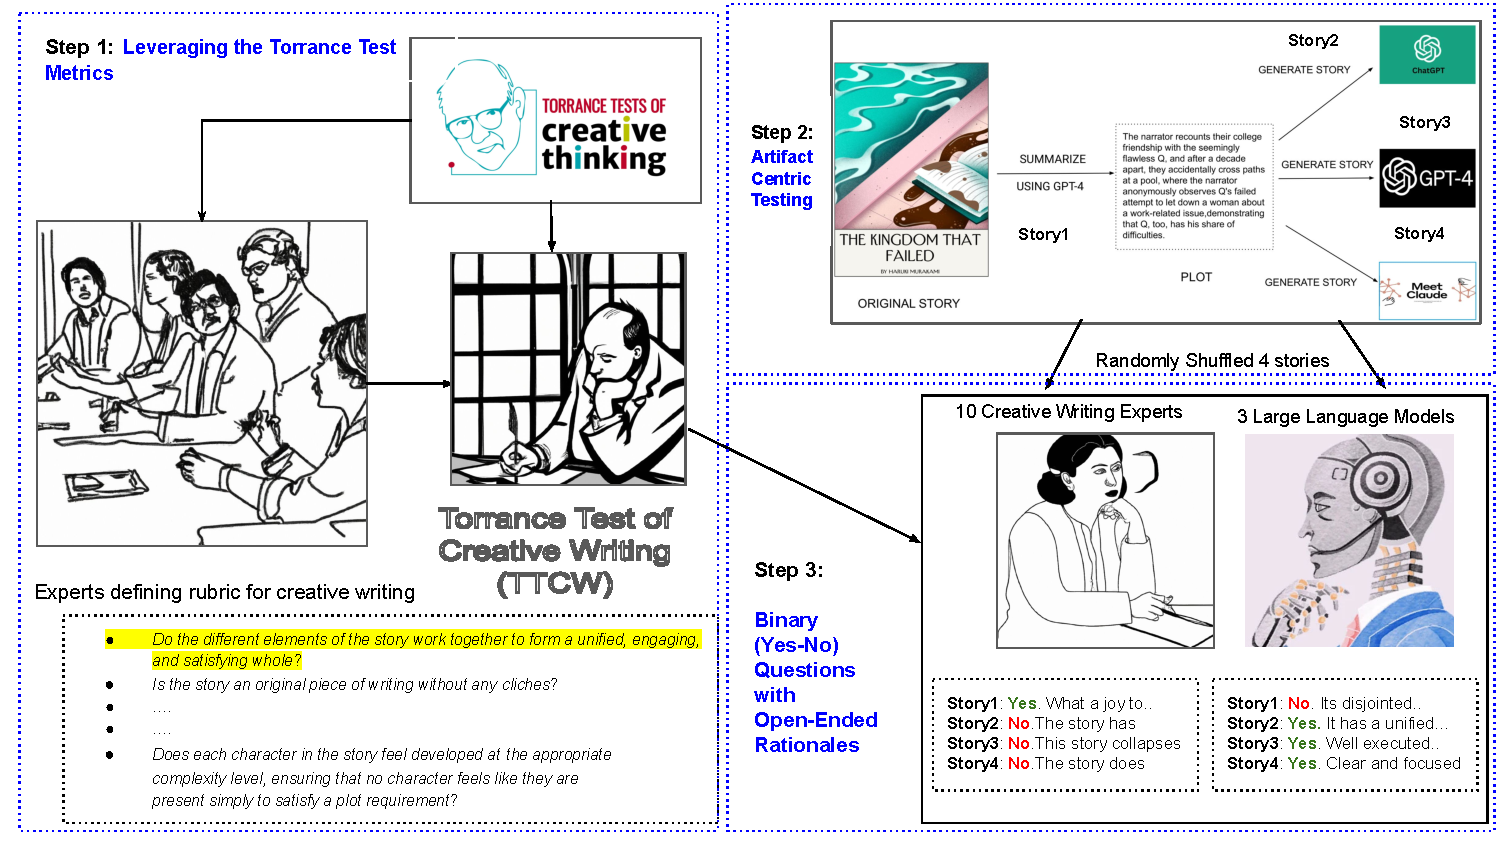
\includegraphics[width=\textwidth]{figures/CHI_pipeline.pdf}
\caption{\label{pipeline}Pipeline showing the construction of TTCW and evaluation of short stories using the TTCW framework}
\end{figure*}

The analysis of the conducted tests reveals that the 12 expert-written stories pass an average of 84.7\% of the tests, confirming that although an expert story must not pass all tests to be deemed creative, experienced writers typically produce artifacts that pass the majority of the tests. In comparison, LLM-generated stories pass many fewer tests on average, from 9\% for ChatGPT-generated~\footnote{\url{https://openai.com}} stories, up to 30\% for Claude-generated~\footnote{\url{https://www.anthropic.com}} stories. In other words, LLM-generated stories are three to ten times less likely to pass individual TTCW tests compared to expert-written stories, revealing a wide gap in the evaluated creativity of LLM-generated content. Besides the general gap, the granularity of the TTCW reveals that individual LLMs differ in abilities, with GPT4 more likely to pass tests associated with Originality, and Claude V1.3 more likely to pass tests in Fluency, Flexibility and Elaboration.

Prior work has argued that even though LLMs might not be able to produce creative content in an end-to-end fashion, they might be utilized in providing feedback to authors during their writing process \cite{ippolito2022creative}. To this effect, we explore in Section ~\ref{sec:llmeval} whether LLMs can administer individual TTCW tests individually, by expanding each test into a detailed prompt, and measuring whether LLM assessments correlate with collected expert judgments. Our analysis reveals that for the most part, LLMs are not capable of administering the TTCW tests, as the three LLMs we experiment with -- ChatGPT, GPT4, and Claude 1.3 -- achieve correlations with experts that are close to zero.

In summary, our work makes the following contributions:
\begin{itemize}
    \item We adapt the Torrance Test for Creative Thinking (TTCT), a framework for evaluating creativity as a process, and align it for the evaluation of creativity as a product particularly focusing on short stories. We design 14 tests called the \textit{Torrance Test for Creative Writing (TTCW)} based on the four original Torrance dimensions of Fluency. Flexibility, Originality, and Elaboration,
    \item We experimentally validate the TTCW through a large-scale assessment of 48 stories involving 10 participants with expertise in creative writing, finding that they reach moderate agreement when administering individual tests, and strong agreement when evaluating all tests in aggregate.
    \item We study the abilities of LLMs to generate stories that pass/fail the TTCW tests and their ability to reliably assess the creativity of stories following the TTCW framework through correlation with human judgments. Our findings show that LLM-generated stories are three to ten times less likely to pass TTCW tests compared to expert-written stories, as well as the fact that current state-of-the-art LLMs are not yet capable of reproducing expert assessments when administering TTCW tests. To enable future research in this fast-evolving domain, we plan to release the large-scale annotation of 2,000+ TTCW assessments, each accompanied with a natural language expert explanation. 
    \item Finally, we discuss how creative writing experts can distinguish between AI v.s. human written stories and how future work can use our evaluation framework for building rich interactive writing support tools.
\end{itemize}
